\section{Results}
\input{./text/Results}

\lipsum

\begin{mcfigure}
	\centering
	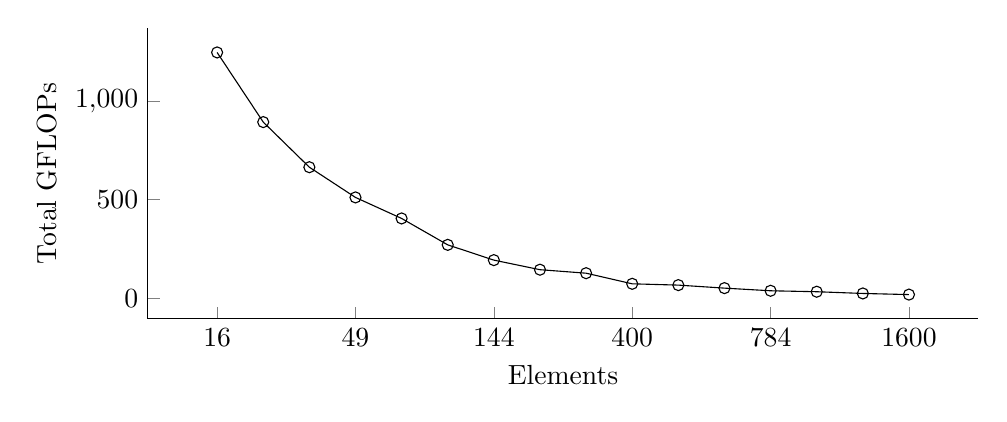
\begin{tikzpicture}
    \begin{axis}[
        height=15em,
        width=\linewidth,
        axis x line*=bottom,
        axis y line*=left,
        symbolic x coords = {16, 25, 36, 49, 64, 100, 144, 196, 225, 400, 441, 576, 784, 900, 1225, 1600},
        xtick = {16, 49, 144, 400, 784, 1600},
        ytick = {0, 500, 1000, 1500},
        domain = 16:1600,
        range = 0:1500,
        xlabel={Elements},
        ylabel={Total GFLOPs}]
        \addplot[
            mark=o,
            color=black] coordinates {
            	(16, 1244.6784)
            	(25, 892.1854771)
            	(36, 663.82848)
            	(49, 510.93504)
            	(64, 404.52048)
            	(100, 270.8420198)
            	(144, 193.61664)             	 
            	(196, 145.152) 
            	(225, 127.4550682) 
            	(400, 73.68496128) 
            	(441, 67.09248) 
            	(576, 51.8616) 
            	(784, 38.46528) 
            	(900, 33.63397632) 
            	(1225, 24.89647104)
            	(1600, 19.16804736)		
            };
    \end{axis}
\end{tikzpicture}

            

	\captionof{figure}{Total FLOPs used to compute the factorized matrix multiplication in $\textbf{F}^{\intercal} \times (\textbf{M}^{-1} \textbf{F})$ over the number of elements for a constant problem size, $N = 705\kern 0.25em 600$. FLOPs decrease as the size of the constituent inner products decrease in relation to the size of each element.}
\end{mcfigure}


\begin{mcfigure}
	\centering
	\begin{tikzpicture}
    \begin{axis}[
        height=2.5in,
        width=3.375in,
        axis x line*=bottom,
        axis y line*=left,
        symbolic x coords = {49, 64, 100, 144, 196, 225, 400, 441, 576, 784, 900, 1225, 1600},
        xtick = {49, 144, 400, 784, 1600},
        ytick distance=20,
        domain = 49:1600,
        range = 0:60,
        xlabel={Elements},
        ylabel={Runtime (s)}]
        \addplot[dashed, 
            mark=x,
            color=violet] coordinates {
            	(49, 58.048654)
            	(64, 44.608081)
            	(100, 30.117423)
            	(144, 22.058077)             	 
            	(196, 16.56574) 
            	(225, 14.797055) 
            	(400, 9.426228) 
            	(441, 8.84558) 
            	(576, 7.915462) 
            	(784, 8.569443) 
            	(900, 9.894469) 
            	(1225, 16.662268)
            	(1600, 32.297395)		
            };                                      
        \addplot[dashed, 
            mark=triangle,
            color=blue] coordinates {
            	(49, 7.159366)
            	(64, 7.466476)
            	(100, 8.700982)
            	(144, 10.472512)             	 
            	(196, 11.721377) 
            	(225, 11.966759) 
            	(400, 14.197423) 
            	(441, 14.494765) 
            	(576, 14.587827) 
            	(784, 15.465336) 
            	(900, 15.557051) 
            	(1225, 16.686761)
            	(1600, 19.131444)		
            };
        \addplot[dashed, 
            mark=+,
            color=red] coordinates {
            	(49, 3.739837)
            	(64, 4.359711)
            	(100, 5.000516)
            	(144, 6.416801)             	 
            	(196, 8.051781) 
            	(225, 9.404944)
            	(400, 9.965406) 
            	(441, 13.815412) 
            	(576, 16.399836) 
            	(784, 19.31444) 
            	(900, 20.800298) 
            	(1225, 24.993118)
            	(1600, 29.029143)		
            };

        \addplot[
            mark=o,
            color=black] coordinates {
                (49, 69.749697)
                (64, 57.215341)
                (100, 45.317181)
                (144, 40.655649)             
                (196, 37.752682)
                (225, 36.783105)
                (400, 37.477622)
                (441, 37.671921)
                (576, 38.931754)
                (784, 43.377669)
                (900, 46.279928)
                (1225, 58.368563)
                (1600, 80.487622)
            };

        \addlegendentry{$\textbf{F}^{\intercal} \textbf{M}^{-1} \textbf{F}$}
        \addlegendentry{Style 2}
        \addlegendentry{$\text{solve}(\lambda_A, \lambda_b)$}
        \addlegendentry{Total TTS}

    \end{axis}
\end{tikzpicture}
\end{mcfigure}